\chapter{Introduction}
\label{sec:introduction}

\section{Background}
\label{sec:introduction:background}

With the rising importance of machine learning in general, the issue of interpretability has gained prominence in recent years~\cite{carvalho2019machine, gilpin2018explaining, molnar2020interpretable}.
In particular, interpretability considers the user perspective, going beyond prediction performance as the only quality criterion for machine-learning approaches.
There are various ways to foster interpretability in machine-learning pipelines.
Two important fields in this direction are feature selection and subgroup discovery.
We will briefly and informally introduce these two fields next; see Chapter~\ref{sec:fundamentals} for detailed fundamentals.

\paragraph{Feature selection}

Feature selection aims to identify the variables in a dataset that are most useful for predictions~\cite{guyon2003introduction}.
Some feature-selection methods act as a pre-processing step before training a prediction model, while others operate during or in combination with model training.
Several reasons speak for feature selection~\cite{chandrashekar2014survey, li2017feature}:
By reducing dataset dimensionality, it lowers the computational cost and memory requirements of training, storing, and using prediction models.
Next, prediction models may generalize better without irrelevant and spurious predictors.
While some model types can implicitly select relevant features, others cannot.
Finally, prediction models with fewer inputs may become simpler, thereby improving interpretability.

\begin{figure}[t]
	\centering
	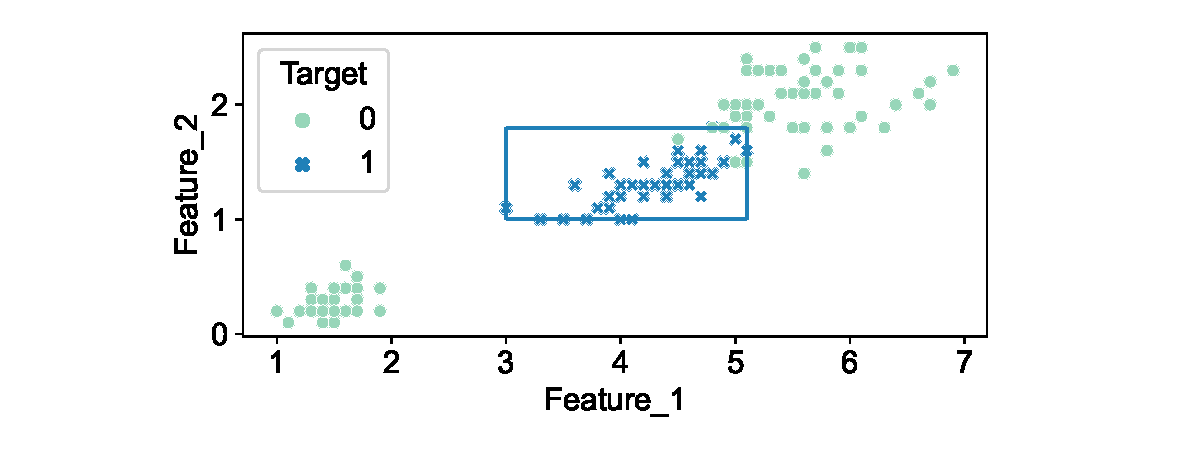
\includegraphics[width=\textwidth, trim=15 15 15 15, clip]{plots/csd-exemplary-subgroup.pdf}
	\caption{
		Exemplary subgroup description in the form of a rectangle for a dataset with two real-valued features and a binary prediction target.
	}
	\label{fig:csd:exemplary-subgroup}
\end{figure}

\paragraph{Subgroup discovery}

The goal of subgroup discovery is to find `interesting' subgroups, i.e., subsets of a dataset, like data objects where the prediction target takes a particular value~\cite{atzmueller2015subgroup}.
Additionally, such subgroups should be described with a combination of simple conditions on feature values, thereby fostering interpretability.
E.g., Figure~\ref{fig:csd:exemplary-subgroup} displays a rectangle-shaped subgroup description for a two-dimensional, real-valued dataset with a binary prediction target.
This subgroup is defined by $(\mathit{Feature\_1} \in [3.0, 5.1]) \land (\mathit{Feature\_2} \in [1.0, 1.8])$ and contains a considerably higher fraction of data objects with $\mathit{Target} = 1$ than the complete dataset.
One may see subgroup discovery as an extension of feature selection.
In particular, the result of subgroup discovery is not only a feature set but also comprises the value conditions.
Instead of training a prediction model with the selected feature set, the subgroup description implicitly forms a prediction model already.
In general, the subgroup description may define conditions on all features.
However, if it becomes too complex, i.e., involves too many features, its interpretability may decrease~\cite{meeng2021real}.
Thus, it makes sense to only use a subset of features in the subgroup description.

\section{Research Gaps}
\label{sec:introduction:research-gaps}

There are many existing methods for feature selection and subgroup discovery~\cite{atzmueller2015subgroup, li2017feature}.
However, we see two main research gaps where these two fields can be made more user-centric:
integrating domain knowledge and finding alternative solutions.
We will elaborate on these two points next.
Additionally, we will explain how we address both points with constraints on feature sets.

\subsection{Integrating Domain Knowledge}
\label{sec:introduction:research-gaps:integrating-domain-knowledge}

\paragraph{Motivation}

Most methods for feature selection and subgroup discovery optimize a quantitative quality criterion, e.g., a metric for prediction performance.
However, such approaches may yield suboptimal results from the user perspective, e.g., for interpreting the feature sets qualitatively.
In particular, these methods disregard domain knowledge about the dataset and its features.
Such domain knowledge is available in many scientific settings~\cite{karpatne2017theory, wagner2016theory}.
Users may want to consider different types of knowledge:
%
\begin{enumerate}
	\item
	\emph{Firm domain knowledge:}
	To make prediction models consistent with the domain, users may want them to adhere to known facts from the domain.
	For example, users may \emph{know} that some features are redundant from the domain perspective and thus want to rule out selecting combinations of these features.
	\item
	\emph{Hypotheses:}
	Hypotheses are ideas or expectations that users would like the selected feature sets to respect.
	For example, users may \emph{hypothesize} that certain features are redundant, and they want to study whether feature sets without these hypothesized redundancies suffice for predictions.
	If prediction performance drops significantly for feature sets respecting this hypothesis, the hypothesis may be wrong.
	\item
	\emph{Preferences:}
	Besides domain knowledge in the narrow sense, users may have further preferences on the selected feature sets.
	One example, which is already common in feature selection and subgroup discovery, is limiting the size of the feature sets.
	In particular, smaller feature sets may be easier to interpret.
\end{enumerate}

\paragraph{Problem and challenges}

In all previous scenarios, users want to limit the space of valid feature sets but not select individual feature sets manually.
Thus, we propose constraints on feature sets as a suitable approach to consider domain knowledge automatically.
We call the corresponding paradigms \emph{constrained feature selection} and \emph{constrained subgroup discovery}.
While observing constraints, we still want to optimize the quality of solutions, i.e., feature sets or subgroups.
The constraints may lower solution quality, but their exact impact is unclear a priori, and a certain decrease may still be acceptable for users.
Another central question is how to consider these constraints.
An ideal approach should support a wide range of constraints and their combination.
This flexibility gives users a lot of freedom, but it makes integration into existing methods for feature selection or subgroup discovery harder.
Also, the approach for integrating constraints should not be tied to one particular method.
I.e., we see the paradigm of constraints as orthogonal to existing methods.
However, the latter differ considerably in their objectives and internal structure, which poses a challenge for integrating constraints in a general fashion.

\paragraph{Related work}

Constraints have been used in many areas of data mining and machine learning~\cite{grossi2017survey}, e.g., automated machine learning~\cite{neutatz2023automl}, clustering \cite{dao2013declarative, dao2024review}, explainable AI~\cite{deutch2019constraints, gorji2022sufficient,  mothilal2020explaining, shrotri2022constraint}, and pattern mining \cite{ng1998exploratory, silva2016constrained}.
In feature selection, existing works tend to aim at just one feature-selection method and one constraint type, like group constraints \cite{friedman2010note, jacob2009group, simon2013sparse, yuan2006model, zhao2006grouped}, cost constraints \cite{jagdhuber2020cost, momeni2021cafs, paclik2002feature, plasberg2009feature, zhang2016learning}, or cardinality constraints \cite{khushaba2011feature, lee2018effective, serpico2001new, yang2015budget}.
Thus, there is potential for a more general approach to constrained feature selection.
In subgroup discovery, considering constraints is more common~\cite{atzmueller2015subgroup, meeng2021real}.
However, the subgroup-discovery methods that support constraints are typically limited to individual constraint types or at least require constraints to have particular properties, since the constraints need to be integrated into algorithmic search procedures.

\subsection{Finding Alternative Solutions}
\label{sec:introduction:research-gaps:finding-alternative-solutions}

\paragraph{Motivation}

Most methods for feature selection and subgroup discovery return only one solution, i.e., the optimum according to a quality criterion.
Nevertheless, there may be different solutions, i.e., using other features, that achieve similar quality.
Such alternative solutions are interesting for users, e.g., to obtain several diverse explanations.
In particular, alternatives can provide additional insights into predictions, enable users to develop and test different hypotheses, appeal to different kinds of users, and foster trust in the predictions~\cite{kim2021multi, wang2019designing}.
For example, in a dataset describing physical experiments, feature selection may help discover relationships between physical quantities.
If multiple alternative sets of similar quality exist, further analyses and experiments may be necessary to reveal the true underlying physical mechanism.
Only knowing one high-quality feature set and using it as the only explanation may be misleading in such a situation.

\paragraph{Problem and challenges}

We call our paradigms for finding alternative solutions \emph{alternative feature selection} and \emph{alternative subgroup description discovery}.
In the former case, we want to optimize feature-set quality; in the latter case, similarity regarding the set of data objects in the subgroup.
In both cases, constraints should enforce that the solutions are alternative in the sense of using different features.
For example, one can search for multiple solutions sequentially and require each new solution to optimize quality while being sufficiently dissimilar to previous solutions.
The constraints should be domain-independent since obtaining alternatives is a general concern and we want to free users from manually formulating corresponding constraint types.
However, users should have control over alternatives, e.g., their number and dissimilarity.
Depending on these user parameters, quality may drop, as with constraints in general, and users should decide on an acceptable quality trade-off.
Another recurring concern is to keep the approach for alternatives orthogonal to existing methods for feature selection and subgroup discovery.

\paragraph{Related work}

Only a few feature-selection methods return multiple, diverse feature sets~\cite{borboudakis2021extending}.
Existing approaches often do not guarantee diversity or do not give users control over diversity.
In fields related to feature selection, the goal of obtaining multiple, diverse solutions has been studied, e.g., for subspace clustering~\cite{hu2018subspace, mueller2009relevant}, subspace search~\cite{trittenbach2019dimension}, or explainable-AI techniques~\cite{artelt2022even, kim2016examples, mothilal2020explaining, russell2019efficient}.
These approaches are not directly applicable or easily adaptable to feature selection, and most of them provide limited or no user control.
In subgroup discovery, various methods yield a diverse set of subgroups~\cite{belfodil2019fssd, bosc2018anytime, leeuwen2012diverse, lemmerich2010fast, lucas2018ssdp+, proencca2022robust}.
However, this notion of alternatives typically aims to cover different subsets of data objects from the dataset.
In contrast, our notion of alternative subgroup descriptions aims to cover a similar set of data objects as in a given subgroup but with different features in the description.
Finally, for feature selection as well as subgroup discovery, existing work on alternatives typically proposes particular new search algorithms rather than an approach that is orthogonal to existing methods.

\section{Contributions}
\label{sec:introductions:contributions}

This dissertation provides four core contributions to make feature selection more user-centric with the help of constraints.
We address both research gaps from the previous section, i.e., integrating domain knowledge (cf.~Section~\ref{sec:introduction:research-gaps:integrating-domain-knowledge}) and finding alternative solutions (cf.~Section~\ref{sec:introduction:research-gaps:finding-alternative-solutions}).
Each core contribution corresponds to one chapter in the main part of this dissertation and may comprise several sub-contributions:

\paragraph{Evaluating the impact of constraints on feature-selection results (cf.~Chapter~\ref{sec:syn})}

First, we formalize constrained feature selection as an optimization problem.
Our problem definition is independent of the feature-selection method.
We also discuss how to solve this problem.
Second, we systematically analyze the impact of constraints.
To this end, we use datasets from various domains and generate random constraints.
A Satisfiability Modulo Theories (SMT) optimizer finds the optimal feature sets under these constraints.
Such a solver-based approach supports a wide range of constraint types.
We analyze the relationships between various evaluation metrics, describing the constraints and the feature-selection results.
Our experiments show that the impact of constraints strongly depends on the constraint type.
Additionally, we observe a nonlinear effect between the strength of constraints and feature-set quality:
Even if constraints prune a significant fraction of feature sets, the quality may not decrease to the same extent.

\paragraph{Formulating scientific hypotheses as constraints (cf.~Chapter~\ref{sec:ms})}

We conduct a case study in materials science to evaluate the impact of constraints for a concrete use case.
Here, we collaborate with domain experts to formulate constraints.
In particular, the constraints represent preferences and hypotheses from the domain.
We evaluate the hypotheses by analyzing how the corresponding constraints affect feature selection.
Our experiments show little variance in feature-set quality over the constraints, indicating that the data does not contradict the hypotheses.
However, the resulting feature sets differ in their composition, demonstrating that alternative solutions of similar quality exist.

\paragraph{Finding alternative feature sets (cf.~Chapter~\ref{sec:afs})}

First, we formalize alternative feature selection as an optimization problem.
In particular, we define alternatives via 0-1 integer linear constraints on feature sets.
Our approach is orthogonal to the feature-selection method and equips users with two parameters, i.e., the number of alternatives and a dissimilarity threshold.
For multiple alternatives, we consider sequential as well as simultaneous search.
Second, we discuss how to solve this optimization problem.
To that end, we describe how to integrate different categories of existing feature-selection methods into a solver-based search for alternatives.
Third, we analyze the time complexity of the optimization problem.
We show $\mathcal{NP}$-hardness, even for a simple notion of feature-set quality.
Fourth, we propose heuristic search methods that achieve a constant-factor approximation for a particular notion of feature-set quality.
Fifth, we conduct comprehensive experiments with five feature-selection methods, five search methods for alternatives, and varying the two user parameters.
Our experiments demonstrate that users can influence the quality of alternatives:
This quality tends to decrease for more alternatives and a higher dissimilarity threshold.
Runtime-wise, a solver-based sequential search for multiple alternatives is significantly faster than a simultaneous one while yielding a similar quality.
Additionally, our heuristic search methods yield a high quality in negligible runtime.

\paragraph{Discovering spare and alternative subgroup descriptions (cf.~Chapter~\ref{sec:csd})}

First, we formalize subgroup discovery as a Satisfiability Modulo Theories (SMT) optimization problem.
This formulation admits a solver-based search for subgroups and allows integrating constraints.
Second, we formalize two constraint types for this optimization problem.
\emph{Feature-cardinality constraints} limit the number of features used in subgroup descriptions.
\emph{Alternative subgroup descriptions} should use different features as a given subgroup description but cover a similar set of data objects.
Users control the number of alternatives and a dissimilarity threshold.
Third, we describe how to integrate these two constraint types into three existing heuristic search methods and two novel baselines for subgroup discovery.
Fourth, we analyze the time complexity of the subgroup-discovery problem with each of these two constraint types and prove several $\mathcal{NP}$-completeness results.
Fifth, we conduct comprehensive experiments with different experimental scenarios:
no constraints, feature-cardinality constraints, alternative subgroup descriptions, and different solver timeouts.
We observe that subgroups using only a few features already show relatively high quality compared to unconstrained subgroups.
With and without constraints, heuristic search methods yield similar subgroup quality as optimal solutions found by solver-based search, while being considerably faster.

\section{Materials}
\label{sec:introduction:materials}

We publish all code and experimental data for this dissertation under permissive licenses.

We provide the code, implemented in Python, via multiple \href{https://github.com/}{\emph{GitHub}} repositories, which we additionally backed up in the \href{https://archive.softwareheritage.org/}{\emph{Software Heritage archive}}:
%
\begin{itemize}
	\item Chapters~\ref{sec:syn} and~\ref{sec:ms}: \url{https://github.com/Jakob-Bach/Constrained-Filter-Feature-Selection} \newline
	Archived at \href{https://archive.softwareheritage.org/swh:1:dir:d94796f72c48b6f539cf528d0a8969b4ff61d42f;origin=https://github.com/Jakob-Bach/Constrained-Filter-Feature-Selection;visit=swh:1:snp:b9f0471bf7c5d1ee48572d687628ed14c786f901;anchor=swh:1:rev:77e893f8a6e42df004c999d009c2a02c8cdd9c5d}{swh:1:dir:d94796f72c48b6f539cf528d0a8969b4ff61d42f}
	\item Chapter~\ref{sec:afs}: \url{https://github.com/Jakob-Bach/Alternative-Feature-Selection} \newline
	Archived at \href{https://archive.softwareheritage.org/swh:1:dir:1e2b6605040a2151d31a90cde947787e92c98519;origin=https://github.com/Jakob-Bach/Alternative-Feature-Selection;visit=swh:1:snp:1413d85e1a9005d5681ee7dbeae0b4df851780de;anchor=swh:1:rev:14dea32227848c06b1430b6371e100f3d8c74010}{swh:1:dir:1e2b6605040a2151d31a90cde947787e92c98519}
	\item Chapter~\ref{sec:csd}: \url{https://github.com/Jakob-Bach/Constrained-Subgroup-Discovery} \newline
	Archived at \href{https://archive.softwareheritage.org/swh:1:dir:5527bcc4a86a1583e8bedf241f4738fc9b0e535c;origin=https://github.com/Jakob-Bach/Constrained-Subgroup-Discovery;visit=swh:1:snp:8f87dcdf0277985d373245e5a23a128efc861153;anchor=swh:1:rev:0c0e4a978c95d881c4c20eecdd5a1ae12ee08ac3}{swh:1:dir:5527bcc4a86a1583e8bedf241f4738fc9b0e535c}
\end{itemize}
%
We released all repositories under the \href{https://opensource.org/license/MIT}{MIT license}.
Each repository contains detailed instructions on how to reproduce the corresponding experiments.
Also, requirements files specify the versions of all dependencies.
Additionally, we organized all generally applicable functionality of each repository, e.g., methods for alternative feature selection, as a Python package to ease reuse.
The corresponding packages \href{https://pypi.org/project/alfese/}{\emph{alfese}}, \href{https://pypi.org/project/cffs/}{\emph{cffs}}, and \href{https://pypi.org/project/csd/}{\emph{csd}} are publicly available on \href{https://pypi.org}{\emph{PyPI}}.

We provide the experimental data via \href{https://radar.kit.edu}{\emph{RADAR4KIT}} and put it under the \href{https://creativecommons.org/licenses/by/4.0/}{CC-BY 4.0 license}: \url{https://doi.org/10.35097/4kjyeg0z2bxmr6eh}

\section{Prior Works}
\label{sec:introduction:prior-works}

This dissertation bases on the following preprints and publications:
%
\begin{itemize}
	\item \fullcite{bach2022empirical}
	\item \fullcite{bach2022leveraging}
	\item \fullcite{bach2023finding}
	\item \fullcite{bach2024alternative}
	\item \fullcite{bach2024using}
\end{itemize}
%
We have reused these prior works' content but revised it to form a coherent monograph.
In particular, these prior works contain all major contributions of this dissertation.
However, we have extended, rephrased, restructured, or shortened the text in various places.
Algorithms, definitions, equations, figures, notation, propositions, and tables in this dissertation may slightly differ from prior works, e.g., due to harmonization.
The four chapters in the main part of this dissertation explicitly state which prior works they base on.
All other chapters may reuse content from each of these prior works.

\section{Dissertation Outline}
\label{sec:introduction:outline}

The remainder of this dissertation is structured into three parts.

First, we present preliminaries.
Chapter~\ref{sec:fundamentals} describes relevant fundamentals of feature selection and subgroup discovery.
Chapter~\ref{sec:related-work} discusses related work for all our contributions.

The second part of this dissertation is the main part.
It consists of four chapters featuring our contributions.
Chapter~\ref{sec:syn} evaluates the impact of constraints on feature-selection results.
Chapter~\ref{sec:ms} presents a case study where constraints express scientific hypotheses.
Chapter~\ref{sec:afs} uses constraints to find alternative feature sets.
Chapter~\ref{sec:csd} employs constraints to discover sparse and alternative subgroup descriptions.

The third part of this dissertation wraps up our work.
Chapter~\ref{sec:conclusions} summarizes the conclusions, and Chapter~\ref{sec:future-work} discusses future work.
After the bibliography, Appendix~\ref{sec:appendix} contains proofs and technical details not included in the main part of this dissertation.
